%!TEX program = xelatex
\documentclass[UTF8,zihao=5]{ctexart} %ctex包的article


\usepackage[hidelinks]{hyperref}%超链接,自动加到目录里面



\title{{\bfseries\rmfamily\Huge{高等流体力学\hspace{1em}\\第1次阅读报告}}}
\author{周涵宇 2022310984}
\date{}

\usepackage[a4paper]{geometry}
\geometry{left=0.75in,right=0.75in,top=1in,bottom=1in}%纸张大小和页边距

\usepackage[
UseMSWordMultipleLineSpacing,
MSWordLineSpacingMultiple=1.5
]{zhlineskip}%office风格的行间距

\usepackage{fontspec}
\setmainfont{Times New Roman}
\setsansfont{Source Sans Pro}
\setmonofont{Latin Modern Mono}
\setCJKmainfont{SimSun}[AutoFakeBold=true]
% \setCJKmainfont{仿宋}[AutoFakeBold=true]
\setCJKsansfont{黑体}[AutoFakeBold=true]
\setCJKmonofont{DengXian}[AutoFakeBold=true]

\setCJKfamilyfont{kaiti}{楷体}
\newfontfamily\CM{Cambria Math}


% \usepackage{indentfirst} %不工作 怎样调整ctex的段首缩进大小呢

\usepackage{fancyhdr}
\pagestyle{fancy}
\lhead{
    \CJKfamily{kaiti}{
        高等流体力学作业\hspace{6em}
        班级\ \ 航博221\hspace{6em}
        学号\ \ 2022310984\hspace{6em}
        姓名\ \ 周涵宇
        }
}
\chead{}
\rhead{}
\lfoot{}
\cfoot{\thepage}
\rfoot{}
\renewcommand{\headrulewidth}{0.5pt} %改为0pt即可去掉页眉下面的横线
\renewcommand{\footrulewidth}{0pt} %改为0pt即可去掉页脚上面的横线
\setcounter{page}{1}


% \usepackage{bm}

\usepackage{amsmath,amsfonts}
\usepackage{array}
\usepackage{enumitem}
\usepackage{unicode-math}

% \usepackage{titlesec} % it subverts the ctex titles
\usepackage{titletoc}


% titles in toc:
\titlecontents{section}
              [2cm]
              {\sffamily\zihao{5}\mdseries}%
              {\contentslabel{3em}}%
              {}%
              {\titlerule*[0.5pc]{-}\contentspage\hspace*{1cm}}

\titlecontents{subsection}
              [3cm]
              {\rmfamily\mdseries\zihao{5}}%
              {\contentslabel{3em}}%
              {}%
              {\titlerule*[0.5pc]{-}\contentspage\hspace*{1cm}}

\titlecontents{subsubsection}
              [4cm]
              {\rmfamily\mdseries\zihao{5}}%
              {\contentslabel{3em}}%
              {}%
              {\titlerule*[0.5pc]{-}\contentspage\hspace*{1cm}}
\renewcommand*\contentsname{\hfill \sffamily\mdseries 目录 \hfill}

\ctexset{
    section={   
        % name={前面,后面},
        number={\arabic{section}.},
        format=\sffamily\raggedright\zihao{4}\mdseries,
        indent= {0em},
        aftername = \hspace{0.5em},
        beforeskip=1ex,
        afterskip=1ex
    },
    subsection={   
        % name={另一个前面,另一个后面},
        number={\arabic{section}.\arabic{subsection}.}, %如果只用一个数字而非1.1
        format=\rmfamily\raggedright\mdseries\zihao{5},%正体字体,不加粗,main字体,五号字
        indent = {2em}, %缩进
        aftername = \hspace{0.5em},
        beforeskip=1ex,
        afterskip=1ex
    },
    subsubsection={   
        % name={另一个前面,另一个后面},
        number={\arabic{section}.\arabic{subsection}.\arabic{subsubsection}.}, %默认的 1.1.1
        format=\rmfamily\raggedright\mdseries\zihao{5},%无衬线字体,加粗,sans字体,五号字
        indent = {2em}, %缩进
        aftername = \hspace{0.5em},  %名字和标题间插入字符(此处是空白)
        beforeskip=1ex, %空行
        afterskip=1ex
    }
}

\usepackage{float}
\usepackage{graphicx}
\usepackage{multirow}
\usepackage{multicol}
\usepackage{caption}
\usepackage{subcaption}
\usepackage{cite}


%part、section、subsection、subsubsection、paragraph、subparagraph
\newcommand{\bm}[1]{{\mathbf{#1}}}
\newcommand{\trans}[0]{^\mathrm{T}}
\newcommand{\tran}[1]{#1^\mathrm{T}}
\newcommand{\hermi}[0]{^\mathrm{H}}
\newcommand{\conj}[1]{\overline{#1}}
\newcommand*{\av}[1]{\left\langle{#1}\right\rangle}
\newcommand*{\avld}[1]{\frac{\overline{D}#1}{Dt}}
\newcommand*{\pd}[2]{\frac{\partial #1}{\partial #2}}
\newcommand*{\pdcd}[3]{\frac{\partial^2 #1}{\partial #2 \partial #3}}
\newcommand*{\inc}[0]{{\Delta}}

\newcommand*{\uu}[0]{\bm{u}}
\newcommand*{\vv}[0]{\bm{v}}
\newcommand*{\g}[0]{\bm{g}}
\newcommand*{\nb}[0]{{\nabla}}



\begin{document}

\maketitle
\thispagestyle{fancy}


% \begin{center}
%     \rmfamily
%     \tableofcontents\setcounter{page}{0}
% \end{center}
% \thispagestyle{empty} % 目录
% \newpage %换页

阅读文献:\\
Cavalieri, André VG, Erico L. Rempel, and Petrônio AS Nogueira. "Transition to chaos in a reduced-order model of a shear layer." Journal of Fluid Mechanics 932 (2022): A43.
\\
剪切层降阶模型的混沌转捩


\section{研究背景和意义}
相干结构是湍流剪切层和射流中的重要特征,
自1970年代初以来已得到一定认识。
在具有类似于转捩流中观察到的K-H涡旋特征的剪切层中会形成大尺度的湍流结构,
这些结构向下游运动,其振幅在空间中增长,
当它们到达具有更厚的剪切层的区域时,
其振幅饱和然后衰减。
这种行为可以被建模为轴向扩展的波包,
这被认为是射流噪声的主要来源。
在湍流射流中,波包在动能方面不是主导结构,
但仍然与远场声音强相关,这是一个已知的过程,与波包的振幅调制或“突跳”有关。

为了建模波包及其声辐射,
通常使用将射流平均场视为基流的线性化模型。
这源自Crighton和Gaster\cite{crighton1976stability}的一个早期想法,
他们通过考虑围绕缓慢扩散的平均流动线性化的运动方程来建模波包。
相干结构被建模为在喷嘴出口激发的Kelvin-Helmholtz波包。
这导致扰动在喷嘴附近呈指数增长,
而随着剪切层变厚,下游振幅衰减。
这些模型的预测导致时间周期性的波包,
与强迫射流实验\cite{cohen1987evolution}
以及最近的自由湍流射流\cite{cavalieri2013wavepackets}有良好的一致性,
尽管在下游区域存在一定的不匹配。

对于湍流剪切流中相干结构的建模,
一种更新的方法是基于解析算子的分析,
采用被视为外部强制项的非线性项强制线性化方程。
该框架涉及到将输入(非线性强制项)和输出(线性化流动响应)进行排序,
这些排名是基于增益(输出能量与输入能量的比率)确定的。
湍流的解析算子分析最初是针对壁面边界流发展起来的,
后来Garnaud等人\cite{garnaud2013preferred}发展了喷流的解析算子模型。
Schmidt\cite{schmidt2018spectral}等人和
Lesshafft\cite{lesshafft2019resolvent}等人对解析算子模式和数值模拟或实验的最近比较表明,
在喷流中,主要响应模式和显著相干结构之间具有良好的一致性。

解析算子分析揭示了非线性项如何激发流的响应,
但是由于非线性项被视为外部强制项,
因此需要进一步分析来理解固有的非线性动力学。
例如,各种相干结构之间的相互作用无法通过解析算子分析以简单的方式进行研究。
通过研究非线性动力学,壁面转捩和湍流流动取得了重大进展,
这研究了如何在层流解的线性稳定性的情况下维持湍流。
一种可行的方法是采用降阶模型,在NS系统的Galerkin投影中考虑少数主导的相干结构。
Galerkin投影导致一个低阶动态系统,显示了相关的非线性相互作用。
该系统可以使用非线性动力学中的通用方法进行检查,
其低维度使得可以快速计算对各种初始条件的响应,从而可以深入研究动力学特性。

近期的研究中,
非线性动力学也使用了直接数值模拟(DNS)的全分辨率计算来研究低雷诺数流动。
对于Couette流动,
自从Nagata\cite{nagata1990three}的开创性工作以来,
研究者已经发现了几个非平凡的稳定和周期解。
这些解是不稳定的,在状态空间中具有鞍点行为。
由于解通过它们的稳定(不稳定)流形吸引(排斥)轨迹,
为状态空间创造了复杂结构,
并且可以通过对包括不变解及其稳定和不稳定流形的适当分析来理解混沌特征\cite{gibson2008visualizing}。
更普遍地说,虽然复杂的流动计算上更具有挑战性,
混沌动力学包括无限不稳定周期解(或轨道),
其吸引和排斥属性可能与混沌吸引子的统计特性相关,
通过周期轨道理论\cite{cvitanovic1989periodic,chandler2013invariant}
可以给出一些结论。

在壁面边界层流中,
由于它们在流向和跨向(或者对于管道流为方位角)两个方向上是均匀的,
降阶模型的推导和不变解的研究就可以极大简化。
这样就可以使用周期边界条件和小的计算域,
即构造所谓的最小流动单元。
总之,波数分解极大地简化了壁面边界层流的分析和建模。
另一方面,圆形喷流只有一个均匀方向,即方位角,
这使得即使是线性分析也更加复杂,需要全局坐标。
与流向不均匀性相关的进一步复杂性在于,喷流动力学和声辐射已知依赖于上游边界层,
这是实验\cite{bridges1987roles}
和数值结果\cite{bogey2010influence}中也可以观察到的。
最近的研究表明,涡旋-喷流包被内部喷嘴边界层结构激发。
这些结构需要包含在湍流喷流的降阶模型中。

在Nogueira&Cavalieri\cite{nogueira2021dynamics}(以下简称NC)中,
与以上方法不同,
通过定义一个在流向方向上均匀的剪切层来避免上游激发问题;
这通过考虑由体积力驱动并由两个水平壁约束的剪切层来实现。
体积力导致速度剖面出现拐点,
导致典型的剪切层和射流的Kelvin-Helmholtz不稳定性,
并且在流向和横向方向上的均匀性导致更简单的相干结构提取和分析它们之间的相互作用。
喷流发散效应被忽略,这有利于动力学系统分析,
因为它允许定义剪切层的最小流动单元;然而,这也带来了一些代价,
因为NC中相干结构中平均流扭曲的影响出现为时间调制,
而不是剪切层和射流中波包的空间调制
\cite{cavalieri2013wavepackets}。

NC研究基于雷诺数为200的DNS,
展示出带有时变KH波振幅调制的极限环振荡。
本文将此流动标记为永久激励、周期性不稳定(PAPU)流,
因为连续的体力使得流动呈现KH不稳定性和稳定性的交替。
振幅调制被证明与时间周期性的平均流扰动有关。
这种扭曲与流动中的卷起、条纹和斜波的振幅有关。
这三个结构经历周期性循环。
DNS的观测促使本文提出一个特定的非线性系统,
类似于Waleffe\cite{waleffe1995transition}提出的边界层湍流模型。
NC中的动力系统定性地再现了极限环的特征,
这使得本文希望额外的建模工作可以进一步了解所涉及的流动。
在这样的简化配置下进行的工作,
使得大多数动力系统理论和混沌的方法都能得到应用,
这有望揭示更复杂的湍流剪切层和喷流的流动特性。
由于剪切层具有易于KH不稳定性的层流解,
因此维持湍流的机制不是主要关注的问题。
对于这样的流动,
非线性动力学可能会揭示各种相干结构的相互作用,
这可能有助于解释湍流流动的特征,
例如前面提到的波包振幅调制和抖动。

在本研究中,本文继续探索NC中的流向均匀剪切层。
与NC中使用的无滑移边界条件不同,
本文考虑壁面的自由滑移条件。
这是因为观察到在NC配置中增加雷诺数会导致出现近壁湍流,
类似于湍流Couette流。
这极大地偏离了所需的平行剪切层行为,
其中壁面应该只起到防止流动扩散的作用。
使用自由滑移边界条件可以避免出现这种近壁波动,正如\cite{chantry2016turbulent}中所示。
此外,使用自由滑移边界条件可以使用傅里叶模式和NS方程的Galerkin投影导出低阶动力学系统。
使用这样简化的模型,动力学特性仍然非常丰富,可以进行详细研究,探索系统的分支和其向混沌行为的转变。
本文的方案突出了条纹、涡旋和斜波之间的相互作用机制,导致涡动抖动。
这为研究更复杂的空间发展剪切层和射流开辟了新的方向。

简而言之,本文通过降阶模型将一个简化的剪切流模型简化为低维的
动力学系统,通过Galerkin投影的选取研究特定的流动模式之间的关系,
以获得对剪切流中湍流和转捩过程非线性混沌效应的认识。
相比于线性模型、数值模拟等手段,这样的方法计算代价小但非线性考虑更多,
能够对相应的流动系统混沌效应更全面地认知。

\section{物理模型与数学建模}

本文的物理模型是源自于\cite{nogueira2021dynamics}的一个简化的平行剪切流,
如图\ref{fig:flow},其中流动不是上游速度差驱动的,而是体积力驱动的。
这样流向和展向都是均匀的。同时,本文进一步认为壁面是自由滑动壁面,
法向速度为0但是切向不限制,这样做的目的是防止出现类似于
边界层的效应而使其更加接近自由剪切流。

\begin{figure}[H]
    \centering
    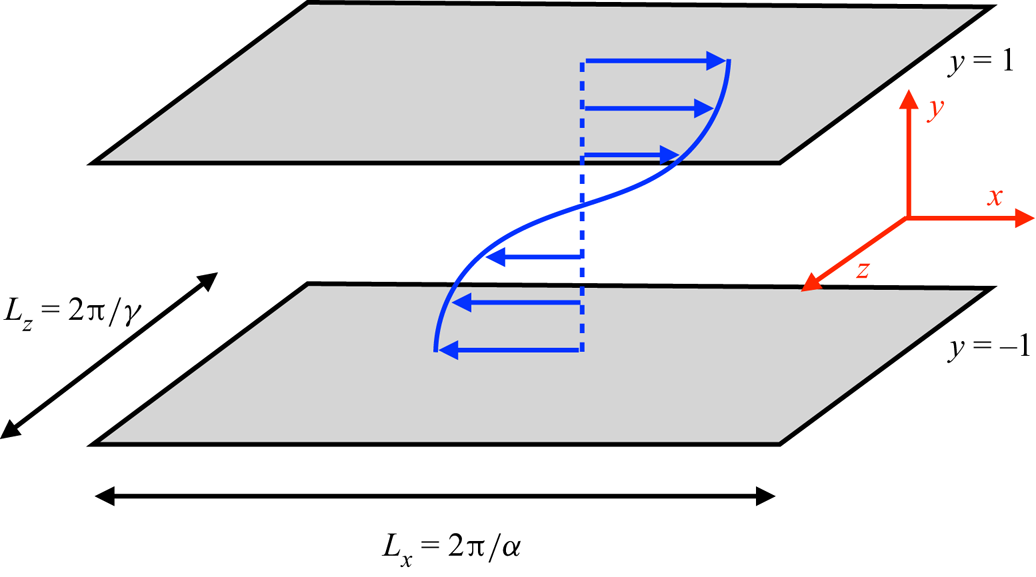
\includegraphics[width=8cm]{flow.png}  %需调整
    \caption{剪切流示意,图中蓝色为体积力}
    \label{fig:flow}
\end{figure}

其中采用不可压NS方程:


\begin{gather} \boldsymbol{\nabla} \boldsymbol{\cdot} \boldsymbol{u}=0, \end{gather}
\begin{gather}\frac{\partial \boldsymbol{u}}{\partial t} + (\boldsymbol{u} \boldsymbol{\cdot} \boldsymbol{\nabla}) \boldsymbol{u} ={-} \boldsymbol{\nabla} p + \frac{1}{{Re}}\nabla^2 \boldsymbol{u} + \boldsymbol{f}, \end{gather}
在$y=\pm 1$的位置形成滑移界面条件。

体积力是:
\begin{equation} \boldsymbol{f} = \frac{\sqrt{2}}{Re} \left(\begin{array}{c} \beta^2 \sin(\beta y)+9 P \beta^2 \sin(3 \beta y)\\ 0\\ 0 \end{array}\right), \end{equation}
其中$\beta=\frac{\pi}{2}$。$P=0$的时候流动比较简单,而$P>0$的时候层流解出现不稳定。
层流解是:
\begin{equation} \boldsymbol{u}_L = \sqrt{2}\left(\begin{array}{c} \sin(\beta y)+P\sin(3\beta y)\\ 0\\ 0 \end{array}\right), \end{equation}
认为扰动在流向和展向是周期的:$(L_x,L_y,L_z)=(2{ \pi} /\alpha, 2, 2{ \pi} / \gamma )$,$\alpha,\gamma$
是流向、展向的主波数。

有了流动单元后,为方便采用Galerkin投影,先定义内积:
\begin{equation} \langle \boldsymbol{f}, \boldsymbol{g} \rangle = \frac{1}{2L_x L_z} \iiint{(f_x g_x + f_yg_y + f_zg_z)\, \mathrm{d}\kern0.7pt x\,\mathrm{d} y\,\mathrm{d}z}, \end{equation}

同时,文章定义了8个互相正交的试函数:
\begin{subequations}
    \begin{gather} \boldsymbol{u}_1 = \left(\begin{array}{c} \sqrt{2} \sin(\beta y)\\ 0\\ 0 \end{array}\right), \end{gather}
    \begin{gather}\boldsymbol{u}_2 = \left(\begin{array}{c} \sqrt{2} \sin(3 \beta y)\\ 0\\ 0 \end{array}\right), \end{gather}
    \begin{gather}\boldsymbol{u}_3 = \left(\begin{array}{c} \dfrac{2 \beta \sin(\alpha x) \sin (\beta y)}{\sqrt{\alpha ^2+\beta ^2}}\\ \dfrac{2 \alpha \cos(\alpha x) \cos(\beta y)}{\sqrt{\alpha^2 +\beta ^2}}\\ 0 \end{array}\right), \end{gather}
    \begin{gather}\boldsymbol{u}_4 = \left(\begin{array}{c} \dfrac{4\beta \cos(\alpha x)\cos(2\beta y)}{\sqrt{\alpha ^2+4\beta^2}}\\ \dfrac{2\alpha \sin(\alpha x)\sin(2\beta y)}{\sqrt{\alpha^2+4 \beta^2}}\\ 0 \end{array}\right), \end{gather}
    \begin{gather}\boldsymbol{u}_5 = \left(\begin{array}{c} 0\\ \dfrac{2 \gamma \cos(\beta y) \sin(\gamma z)}{\sqrt{\beta ^2+\gamma ^2}}\\ -\dfrac{2 \beta \cos(\gamma z) \sin(\beta y)}{\sqrt{\beta ^2+\gamma ^2}} \end{array}\right), \end{gather}
    \begin{gather}\boldsymbol{u}_6 = \left(\begin{array}{c} -\sqrt{2} \sin(\gamma z)\\ 0\\ 0 \end{array}\right), \end{gather}
    \begin{gather}\boldsymbol{u}_7 = \left(\begin{array}{c} \dfrac{2 \gamma \sin(\alpha x) \sin(\gamma z)}{\sqrt{\alpha ^2+\gamma ^2}}\\ 0\\ \dfrac{2 \alpha \cos(\alpha x) \cos(\gamma z)}{\sqrt{\alpha ^2+\gamma ^2}} \end{array}\right), \end{gather}
    \begin{gather}\boldsymbol{u}_8 = \left(\begin{array}{c} \dfrac{2 \sqrt{2} \gamma \cos(\alpha x) \sin(\beta y) \sin(\gamma z)}{\sqrt{\alpha ^2+\gamma ^2}}\\ 0\\ -\dfrac{2 \sqrt{2} \alpha \cos(\gamma z) \sin(\alpha x) \sin(\beta y)}{\sqrt{\alpha ^2+\gamma ^2}} \end{array}\right). \end{gather}
\end{subequations}

其意义可见图\ref{fig:modes}。

\begin{figure}[H]
    \centering
    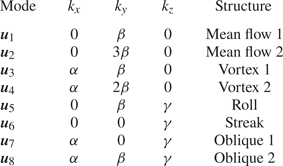
\includegraphics[width=8cm]{modes.png}  %需调整
    \caption{不同模式的含义}
    \label{fig:modes}
\end{figure}

通过不同模式的叠加,
\begin{equation} \boldsymbol{u}(x,y,z,t) = \sum_j {a_j(t) \boldsymbol{u}_j(x,y,z)},\end{equation}
代入NS方程进行Galerkin投影,有如下动力学系统:

\begin{subequations}
    \begin{align} \dot{a}_1 &= \frac{\beta (2 \beta -2 a_{1} \beta )}{2 Re}-\frac{\beta \left(\dfrac{2 a_{5} a_{6} \gamma }{k_{\beta,\gamma}}-\dfrac{3 \sqrt{2} a_{3} a_{4} \alpha \beta }{k_{\alpha,2\beta} k_{\alpha,\beta}}\right)}{2}, \end{align}
    \begin{align}\dot{a}_2 &= \frac{9 \beta ^2 (P-a_{2})}{Re}+\frac{3 \sqrt{2} a_{3} a_{4} \alpha \beta ^2}{2 k_{\alpha,2\beta} k_{\alpha,\beta}}, \end{align}
    \begin{align} \dot{a}_3 &={-}\frac{a_{3} (\alpha ^2+\beta ^2)}{Re}-\frac{\sqrt{2} a_{1} a_{4} \alpha (\alpha ^2+3 \beta ^2)}{2 k_{\alpha,2\beta} k_{\alpha,\beta}}-\frac{\sqrt{2} a_{2} a_{4} \alpha (\alpha ^2-5 \beta ^2)}{2 k_{\alpha,2\beta} k_{\alpha,\beta}} \nonumber\\ &\quad -\frac{2 a_{6} a_{8} \alpha \beta \gamma }{k_{\alpha,\beta} k_{\alpha,\gamma}}-\frac{a_{5} a_{7} \gamma ^2 (\alpha ^2-\beta ^2)}{k_{\alpha,\beta} k_{\alpha,\gamma} k_{\beta,\gamma}}, \end{align}
    \begin{align} \dot{a}_4 &={-}\frac{a_{4} (\alpha ^2+4 \beta ^2)}{Re}+\frac{\sqrt{2} a_{1} a_{3} \alpha ^3}{2 k_{\alpha,2\beta} k_{\alpha,\beta}}+\frac{\sqrt{2} a_{2} a_{3} \alpha (\alpha ^2-8 \beta ^2)}{2 k_{\alpha,2\beta} k_{\alpha,\beta}} \nonumber\\ &\quad +\frac{\sqrt{2} a_{5} a_{8} \gamma ^2 (\alpha ^2-4 \beta ^2)}{2 k_{\alpha,2\beta} k_{\alpha,\gamma} k_{\beta,\gamma}}, \end{align}
    \begin{align} \dot{a}_5 &={-}\frac{a_{5} (\beta ^2+\gamma ^2)}{Re}+\frac{\sqrt{2} a_{4} a_{8} \alpha^2 (\beta ^2-\gamma ^2)}{2 k_{\alpha,2\beta} k_{\alpha,\gamma} k_{\beta,\gamma}}-\frac{a_{3} a_{7} \alpha ^2 (\beta ^2-\gamma ^2)}{k_{\alpha,\beta} k_{\alpha,\gamma} k_{\beta,\gamma}}, \end{align}
    \begin{align}\dot{a}_6 &={-}\frac{a_{6} \gamma ^2}{Re}+\gamma \left(\frac{a_{1} a_{5} \beta }{k_{\beta,\gamma}}+\frac{a_{3} a_{8} \alpha \beta }{k_{\alpha,\beta} k_{\alpha,\gamma}}\right), \end{align}
    \begin{align}\dot{a}_7 &={-}\frac{a_{7} (\alpha ^2+\gamma ^2)}{Re}+a_{1} a_{8} \alpha +\frac{a_{3} a_{5} \beta ^2 (\alpha ^2-\gamma ^2)}{k_{\alpha,\beta} k_{\alpha,\gamma} k_{\beta,\gamma}}, \end{align}
    \begin{align}\dot{a}_8 &={-}\frac{a_{8} (\alpha ^2+\beta ^2+\gamma ^2)}{Re}+\frac{a_{3} a_{6} \alpha \beta \gamma }{k_{\alpha,\beta} k_{\alpha,\gamma}}-a_{1} a_{7} \alpha -\frac{\sqrt{2} a_{4} a_{5} \beta ^2 (\alpha ^2-4 \gamma ^2)}{2 k_{\alpha,2\beta} k_{\alpha,\gamma} k_{\beta,\gamma}}, \end{align}
\label{eq:rom}
\end{subequations}

其中有辅助波数:$k_{i\alpha,j\beta } = \sqrt {(i\alpha) ^2+(j\beta) ^2}, i,j=1,2,3...$,对于$\gamma$同理。

通过\eqref{eq:rom}的降阶模型,可以进行比较细致的计算,探讨动力学系统的混沌特性。

\section{结果与讨论}

雷诺数与$P$都会影响系统的特性。第一次分岔是叉形分岔,如$P=0.08, Re=26.3$的地方,如图\ref{fig:pitchfork}。

\begin{figure}[H]
    \centering
    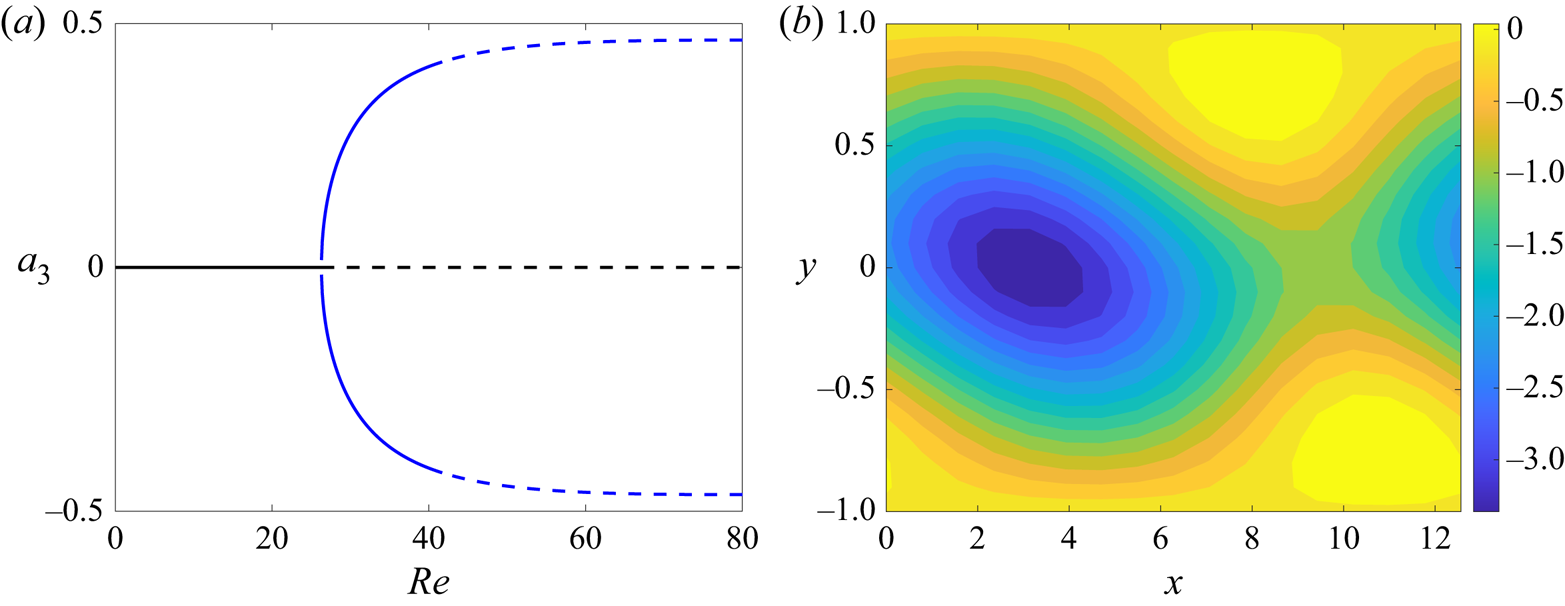
\includegraphics[width=12cm]{pitchfork.png}  %需调整
    \caption{叉形分岔}
    \label{fig:pitchfork}
\end{figure}
分岔后形成图中所示的KH涡,KH涡在雷诺数小于$41.8$的时候都是稳定的。
超过这个雷诺数后,出现超临界的Hopf分岔,分岔后附近出现稳定极限环如图\ref{fig:limitcycle}。
\begin{figure}[H]
    \centering
    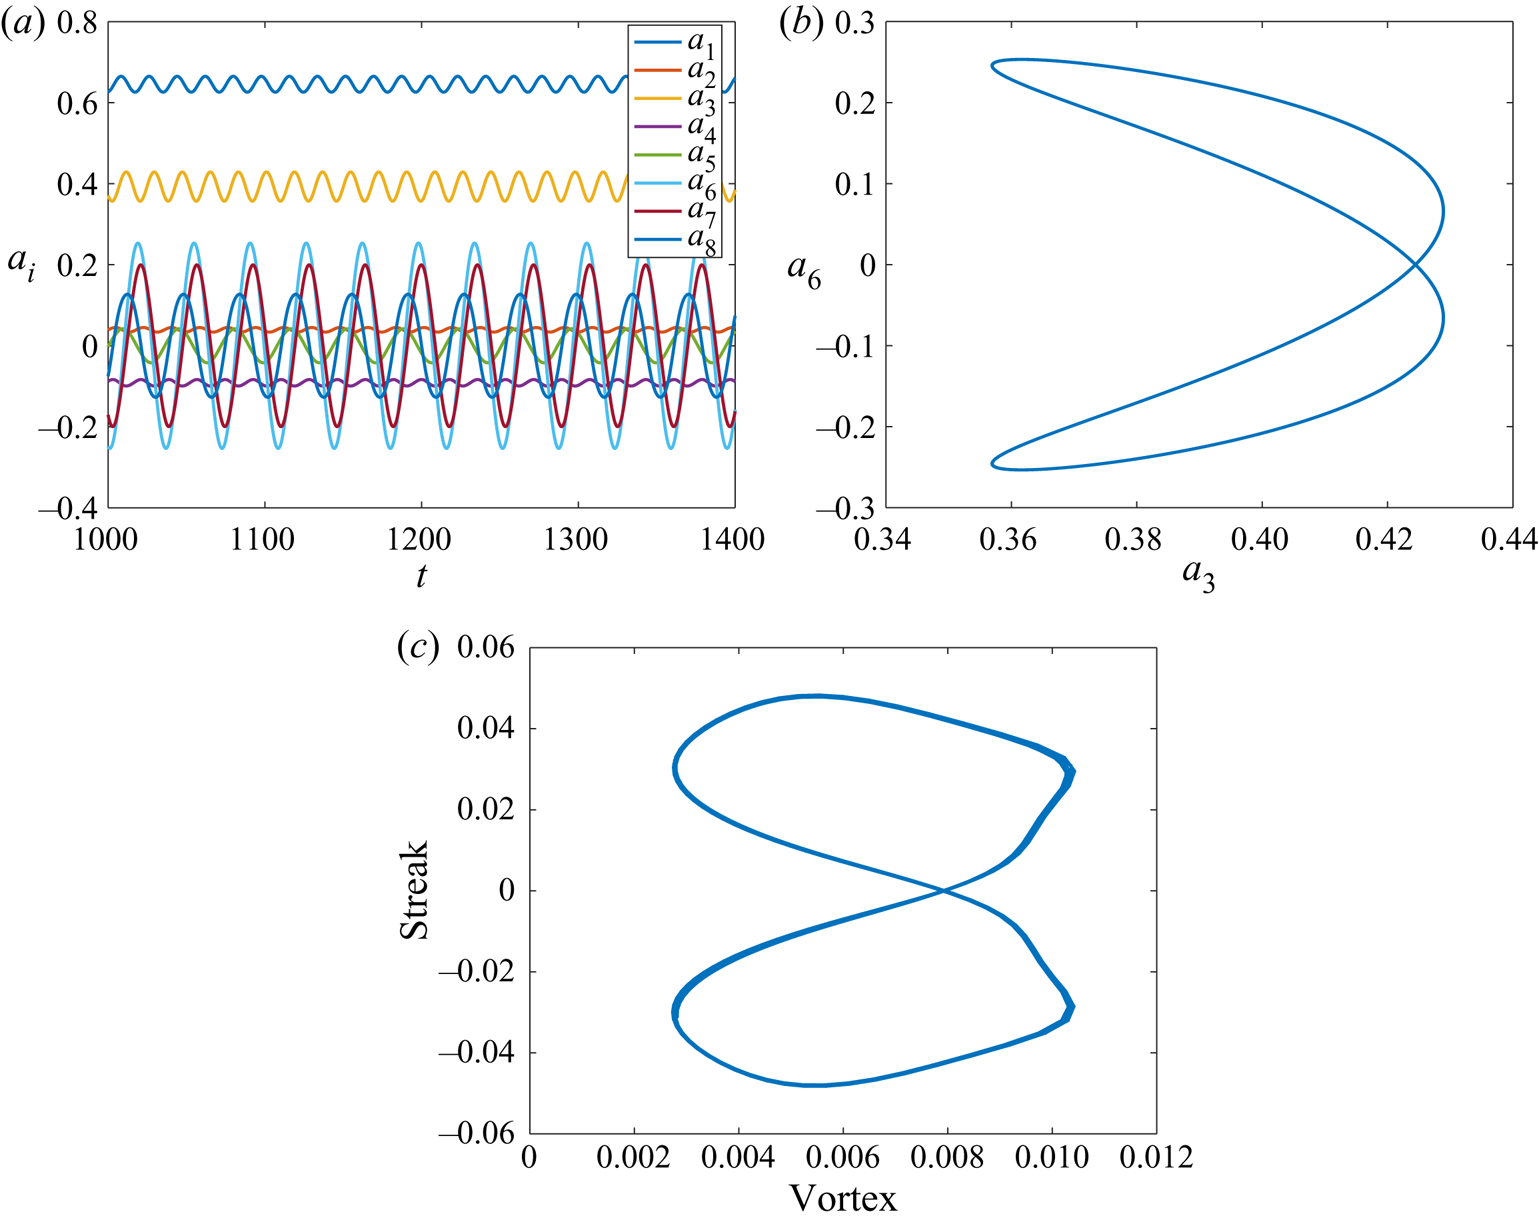
\includegraphics[width=12cm]{limcycle.png}  %需调整
    \caption{极限环Re=50}
    \label{fig:limitcycle}
\end{figure}
关于极限环的细致讨论见原文,包括$Re<120$时的一些Floquet稳定性分析。

在$Re=52$附近出现对称性破缺,$P=0.08, Re=54$的庞加莱截面和相轨迹如图\ref{fig:fig8}。
\begin{figure}[H]
    \centering
    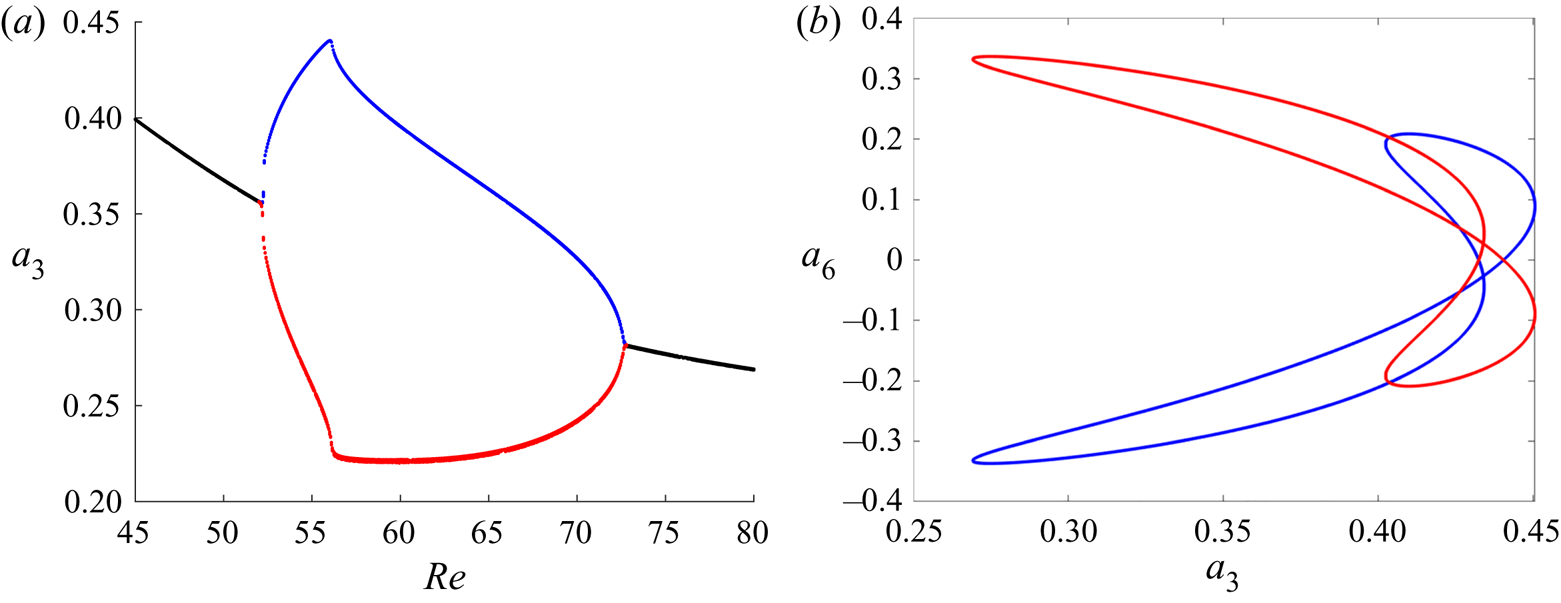
\includegraphics[width=12cm]{fig8.png}  %需调整
    \caption{对称性破缺}
    \label{fig:fig8}
\end{figure}

在雷诺数50、80,存在鞍点,附近处于瞬态混沌,如图\ref{fig:fig9},
其中混沌过后解趋向于周期解。
\begin{figure}[H]
    \centering
    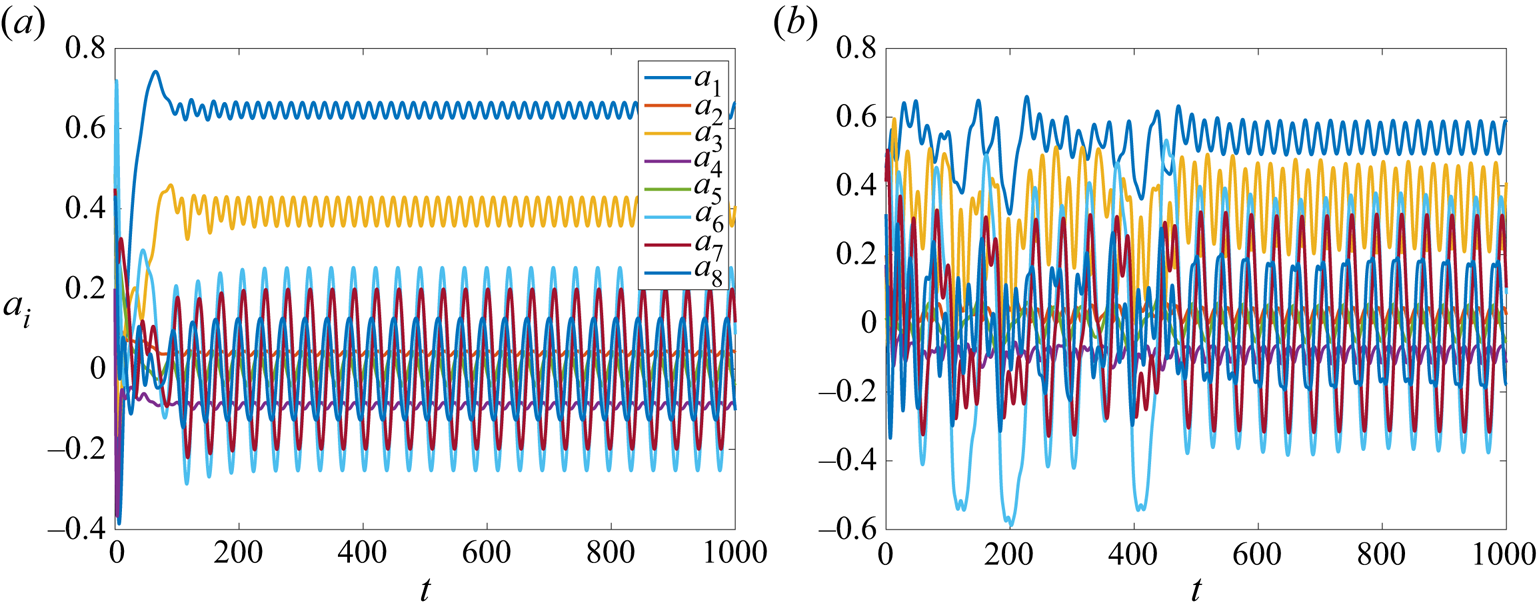
\includegraphics[width=12cm]{fig9.png}  %需调整
    \caption{P=0.08,左Re=50,右Re=80}
    \label{fig:fig9}
\end{figure}

调整不同的P,观察$a_3$法向的庞加莱截面,$Re=54$,如图\ref{fig:fig10}
\begin{figure}[H]
    \centering
    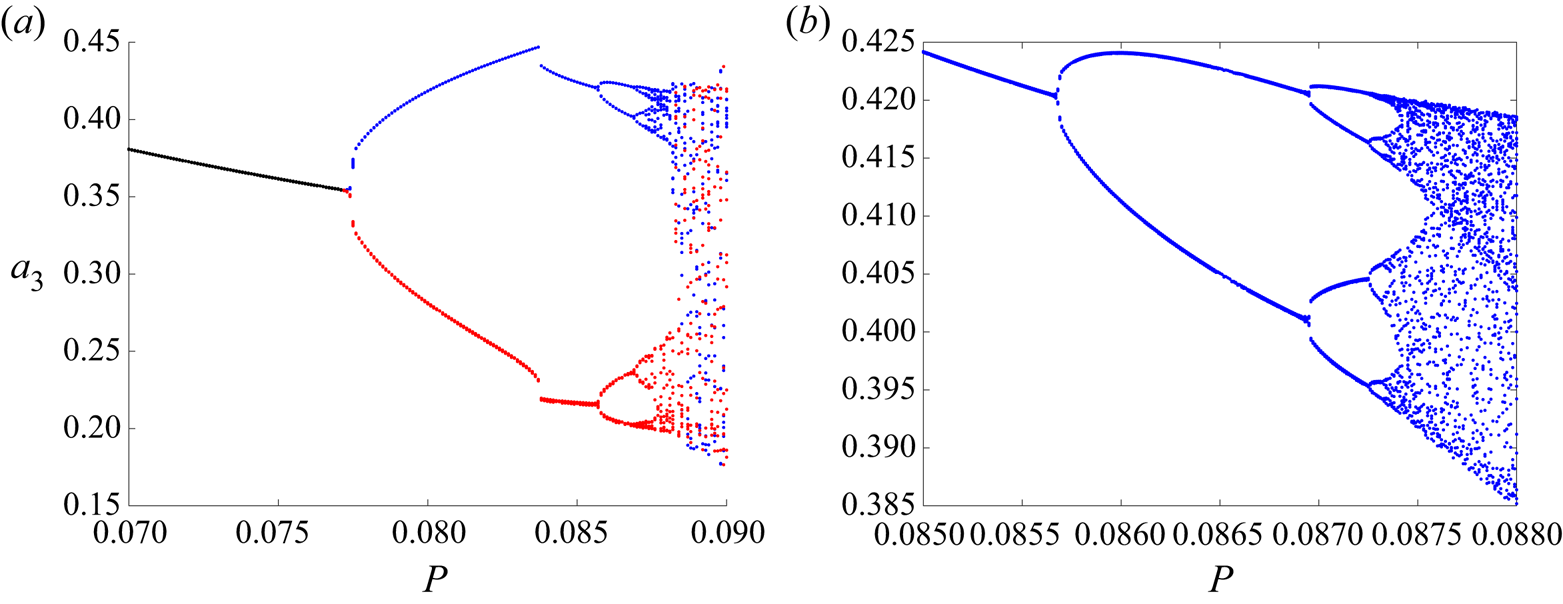
\includegraphics[width=12cm]{fig10.png}  %需调整
    \caption{不同P的庞加莱截面}
    \label{fig:fig10}
\end{figure}

图中可见,$P=0.077$出现对称性破缺的分岔,$P=0.0837$出现了鞍点分岔,
$P\approx0.0874$之后,进入混沌状态。
在$P=0.088$之前,混沌存在两个吸引子,此后出现吸引子的融合,变成1个吸引子。

回到$P=0.08$,存在稳定极限环的情况,增大雷诺数,庞加莱截面
和$Re=130$的相轨迹如图:
\begin{figure}[H]
    \centering
    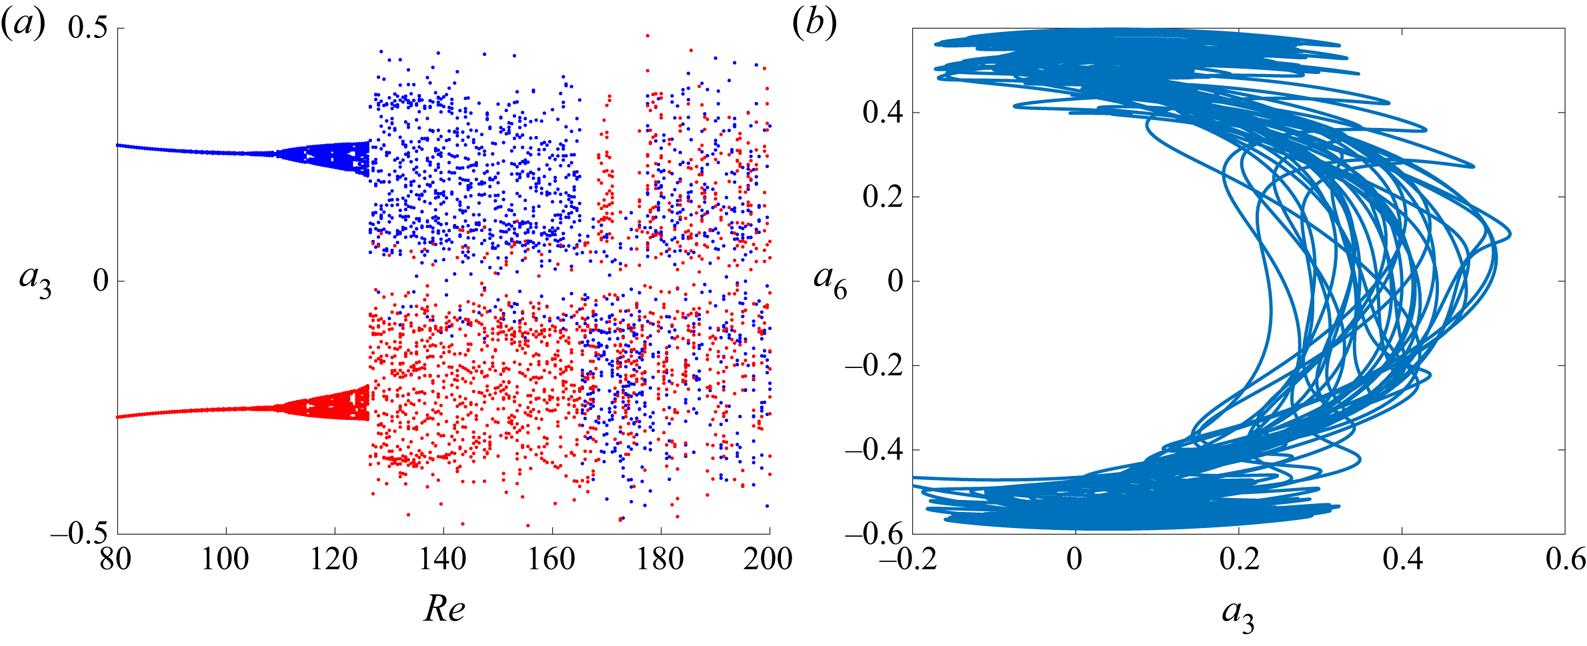
\includegraphics[width=12cm]{fig13.png}  %需调整
    \caption{P=0.08的庞加莱截面和相轨迹}
    \label{fig:fig13}
\end{figure}
图中可见当$Re=109$系统进入准周期吸引子,
文中进一步通过PSD分析了其中的频率成分;
当雷诺数进一步增大到$126.5$以上,转捩为完全的混沌吸引子。
PSD分析显示,准周期时有几个主频和倍频,但是混沌时频谱没有明显的主频。

图\ref{fig:fig13}同时显示了当雷诺数大于$164.5$,混沌吸引子开始融合。
不同雷诺数的相轨迹如图:
\begin{figure}[H]
    \centering
    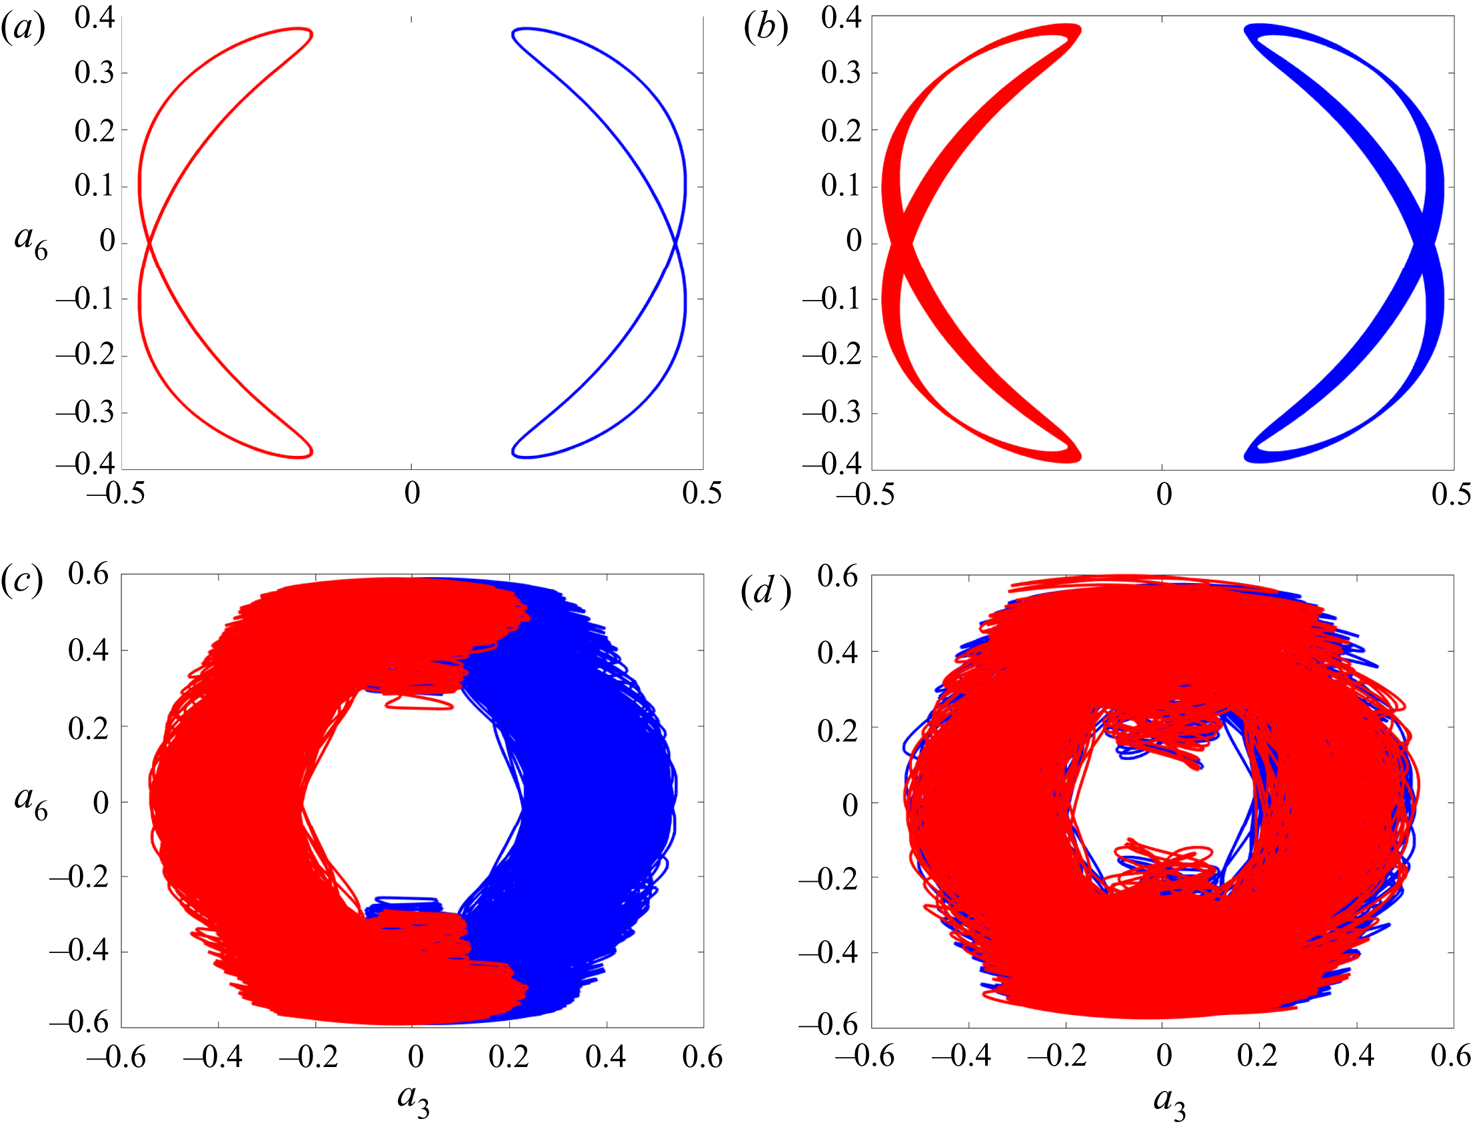
\includegraphics[width=12cm]{fig17.png}  %需调整
    \caption{Re=100,120,150,180的相轨迹}
    \label{fig:fig17}
\end{figure}
可见混沌吸引子出现了融合,轨道不可区分。

\section{总结}

本文通过降阶模型方法,将壁面限制的剪切流动简化为8个模式
的非线性动力学系统,并且研究了其中的失稳、转捩、突跳、混沌、分岔、
准周期、频谱等特性。
研究发现,不同的外力参数P和雷诺数Re会造成系统的不同分岔过程和
吸引子的融合过程。通过这一系列的观察,本文可以成功解释
剪切流中KH波包相位突跳等现象。

本文的主要创新工作是给出了合理的简化物理模型,
并且选取了能够显示流动特征的模态进行Galerkin投影,
得到了充分体现原有系统非线性特性的降阶模型。
同时,本文的分析成功通过降阶模型解释了DNS中观测到的一些混沌现象。

\section{体会与思考}
本文中降阶模型的构造需要选取特定的正交模态,
选取模态选取中最大的特征是,
每一个模态都有一定的物理意义,
可以有选择性地选取主要的流动特征。
这与Bernard对流中有一定的相似之处,
因为Bernard对流中的三个模态,
就体现了速度和温度分布的最基本的几个偏移,
具有较好的代表性。

此外,物理模型的简化也与Bernard对流的工作有一定的相似。
Bernard对流中为了简化,将上下表面定义为自由面,
虽然实际的对流都是无滑移壁面;
而本文中通过给自由剪切流加入了两个滑移壁面的限制,
同样使得问题更加简单,边界条件更容易指定,
从而为降阶模型的分析创造有利条件。

在分析降阶模型的过程中,分析平衡点、庞加莱截面、相轨迹、频谱的方法
是被反复采用的,这些方法可以直观地给出系统的特性范围。在这些分析
方法的基础上,对问题的参数进行分类讨论和计算,就可以得到系统的
主要特征和变化趋势。这些分析中,可视化手段是必不可少的,
很难想象对于如此复杂的系统,
如果不绘制平衡点分布或者庞加莱截面的图形,
怎样找到系统的转捩、分岔特性。

根据本文的思路,进一步的工作可能有,将方法推广到不同
边界条件的问题,探讨边界条件的影响;
或者将方法中部分输入改为数值计算的输入,将过程与部分的DNS融合。
同时,本文展现的分析过程比较繁琐,是否有自动化方法
将整个参数空间中每一点的状态(混沌、极限环等)以及发生的变化(分岔、转捩等)
确定,也是值得研究的,这将大大拓展混沌理论可以应用的系统范围。


\bibliography{refs}{}
\bibliographystyle{unsrt}

% \section*{附录}
% 本文计算代码都在\href{https://github.com/harryzhou2000/HW_ACFD}{Github Repo中(点击访问)}。































% \section{SECTION 节}

% 一个

% \subsection{SUBSECTION 小节}

% 示例

% \subsubsection{SUBSUBSECTION 小节节}

% 字体字号临时调整:
% {
%    \sffamily\bfseries\zihao{3} 哈哈哈哈哈 abcde %三号 sans系列字体(一开始设置的) 加粗
%    %只对大括号范围内的后面的字有用,在标题、题注里面同样
% }
% { 
%    \CJKfamily{kaiti}\zihao{5}\itshape 哈哈哈哈哈 abcde%三号 kaiti(一开始设置的, 斜体(英文有变)
%    %只对大括号范围内的后面的字有用,在标题、题注里面同样
% }

% 一大堆一大堆一大堆一大堆一大堆一大堆一大堆一大堆一大堆一大堆
% 一大堆一大堆一大堆一大堆一大堆一大堆一大堆一大堆一大堆一大堆一大堆一大堆
% 一大堆一大堆一大堆一大堆一大堆一大堆一大堆一大堆一大堆一大堆一大堆一大堆
% 一大堆一大堆一大堆一大堆一大堆一大堆一大堆一大堆一大堆一大堆一大堆一大堆

% \begin{center}
%     居中的什么乱七八糟东西
% \end{center}


% 一个列表:
% \begin{itemize}
%     \item asef
%     \item[\%] asdf
%     \item[\#] aaa
% \end{itemize}

% 一个有序列表:
% \begin{enumerate}
%     \item asef
%     \item[\%\%] asdf
%     \item aaa
% \end{enumerate}

% 一个嵌套列表,考虑缩进:
% \begin{enumerate}[itemindent=2em] %缩进
%     \item asef \par asaf 东西东西东西东西东西东西东西东西东西东西东西东西东西东西东西东西东西东西东西东西东西东西东西东西,
%           F不是不是不是不是不是不是不是不是不是不是不是不是不是不是不是
%           \begin{itemize}[itemindent=2em]  %缩进
%               \item lalala
%               \item mamama
%           \end{itemize}
%     \item asdf
%     \item aaa
% \end{enumerate}

% \section{SECTION}

% 图片排版:

% \begin{figure}[H]
%     \begin{minipage}[c]{0.45\linewidth}  %需调整
%         \centering
%         \includegraphics[width=8cm]{RAM_O2_4660.png}  %需调整
%         \caption{第一个图}
%         \label{fig:a}
%     \end{minipage}
%     \hfill %弹性长度
%     \begin{minipage}[c]{0.45\linewidth}  %需调整
%         \centering
%         \includegraphics[width=8cm]{RAM_O4_4660.png}  %需调整
%         \caption{第二个图}
%         \label{fig:b}
%     \end{minipage}
% \end{figure}

% figure的选项为“htbp”时,会自动浮动,是“H”则和文字顺序严格一些。

% \begin{figure}[H]
%     \begin{minipage}[c]{0.45\linewidth}  %需调整
%         \centering
%         \includegraphics[width=8cm]{RAM_O2_4660.png}  %需调整
%         \label{fig:x}
%     \end{minipage}
%     \hfill %弹性长度
%     \begin{minipage}[c]{0.45\linewidth}  %需调整
%         \centering
%         \includegraphics[width=8cm]{RAM_O4_4660.png}  %需调整
%         \label{fig:y}
%     \end{minipage}
%     \caption{第三个图}
% \end{figure}

% \begin{figure}[H]
%     \centering
%     \includegraphics[width=8cm]{RAM_O4_4660.png}  %需调整
%     \label{fig:c}
%     \caption{第四个图}
% \end{figure}



% \subsection{SUBSECTION}

% 关于怎么搞表格:

% \begin{table*}[htbp]
%     \footnotesize
%     \begin{center}
%         \caption{一端力矩载荷下的结果\fontsize{0pt}{2em}} %需要学习统一设置;0代表不变?
%         \label{表2}
%         \begin{tabular}{|c|c|c|c|c|c|c|}
%             \hline
%             节点数                              & 积分方案              & 单元数                & $h=1m$                & $h=0.1m$              & $h=0.05m$             & $h=0.01m$             \\
%             \hline
%             \multirow{6}{*}{2}                  & \multirow{3}{*}{精确} & 1                     & 4.235294117647059E-08 & 1.406250000000000E-06 & 2.862823061630218E-06 & 1.439654482924097E-05 \\
%             \cline{3-7}
%                                                 &                       & 10                    & 5.975103734439814E-08 & 4.235294117646719E-05 & 1.800000000000410E-04 & 1.406249999999849E-03 \\
%             \cline{3-7}
%                                                 &                       &
%             10000                               & 5.999999915514277E-08 & 5.999996622448291E-05 & 4.799989509752562E-04 & 5.999793702477535E-02                                                 \\
%             \cline{2-7}
%                                                 & \multirow{3}{*}{减缩} & 1                     & 6.000000000000001E-08 & 5.999999999999972E-05 & 4.799999999999911E-04 & 6.000000000003492E-02 \\
%             \cline{3-7}
%                                                 &                       & 10                    & 6.000000000000071E-08 & 5.999999999999142E-05 & 4.799999999995399E-04 & 5.999999999903294E-02 \\
%             \cline{3-7}
%                                                 &                       & 10000                 & 6.000000112649221E-08 & 5.999999234537814E-05 & 4.799997501925065E-04 & 6.000037607984510E-02 \\
%             \hline

%             \multirow{6}{*}{3}                  & \multirow{3}{*}{精确} & 1                     & 6.000000000000003E-08 & 6.000000000000202E-05 & 4.800000000000831E-04 & 6.000000000056749E-02 \\
%             \cline{3-7}
%                                                 &                       & 10                    & 5.999999999999932E-08 & 6.000000000004190E-05 & 4.800000000000206E-04 & 6.000000001613761E-02 \\
%             \cline{3-7}
%                                                 &                       & 10000                 & 6.000000013769874E-08 & 5.999989495410481E-05 & 4.799942099727246E-04 & 6.000263852944890E-02 \\
%             \cline{2-7}
%                                                 & \multirow{3}{*}{减缩} & 1                     & 6.000000000000002E-08 & 6.000000000000267E-05 & 4.800000000000754E-04 & 5.999999999989982E-02 \\
%             \cline{3-7}
%                                                 &                       & 10                    & 5.999999999999899E-08 & 5.999999999987338E-05 & 4.799999999947916E-04 & 5.999999998625345E-02 \\
%             \cline{3-7}
%                                                 &                       & 10000                 & 5.999999728157785E-08 & 5.999994914321980E-05 & 4.800008377474699E-04 & 5.999472246346305E-02 \\
%             \hline

%             \multicolumn{3}{|c|}{欧拉-伯努利解} & 6.000000000000000E-08 & 6.000000000000000E-05 & 4.800000000000000E-04 & 6.000000000000000E-02                                                 \\
%             \hline
%         \end{tabular}
%     \end{center}
% \end{table*}

% 多行、多列表格的示例,基本思想是,多列的那个东西放在多列的最上面一格,下面的行要用\&来空开,也就是\&的数目
% 和普通表格一样,是列数减一;
% 多列的部分的话,就是每行内的操作,相应的\&就少了,见最后一行。

% tabular的“|c|c|c|c|c|c|c|”,意思是,竖线-居中-竖线-居中-竖线……,可以选择省略一些竖线;
% 每行之间的hline,代表贯通的横线,cline是有范围的横线。

% \subsubsection{SUBSUBSECTION}

% newcommand可以用来定义新指令,似乎基本上就是字符串替换……不太懂,总之在公式里面可以用,
% 外面也经常用。






% 公式这么写:
% \begin{equation}
%     \begin{aligned}
%         \frac{aa(x^1+x^2)}{\sqrt{x^1x^2}}
%         \nabla\times\uu
%         = & u_{j;m}\g^m\times\g^j
%         =u_{j;m}\epsilon^{mjk}\g_k
%         =u_{j,m}\epsilon^{mjk}\g_k                           \\
%         = & \frac{1}{\sqrt{g}}\left|
%         \begin{matrix}
%             \g_1       & \g_2       & \g_3       \\
%             \partial_1 & \partial_2 & \partial_3 \\
%             u_1        & u_2        & u_3
%         \end{matrix}
%         \right|
%         =\frac{\sqrt{x^1x^2}}{aa(x^1+x^2)}
%         \left|
%         \begin{matrix}
%             \g_1                        & \g_2                        & \g_3       \\
%             \partial_1                  & \partial_2                  & \partial_3 \\
%             u^1\frac{a^2(x^1+x^2)}{x^1} & u^2\frac{a^2(x^1+x^2)}{x^2} & u^3
%         \end{matrix}
%         \right|                                              \\
%         = & \frac{\sqrt{x^1x^2}}{aa(x^1+x^2)}
%         [[\g_1\,\g_2\,\g_3]]
%         diag\left(
%         u^3_{,2}-u^2_{,3}\frac{a^2(x^1+x^2)}{x^2},\,
%         u^1_{,3}\frac{a^2(x^1+x^2)}{x^1}-u^3_{,1},\, \right. \\
%           & \left.
%         u^2_{,1}\frac{a^2(x^1+x^2)}{x^2}+u^2\frac{a^2}{x^2}
%         -
%         u^1_{,2}\frac{a^2(x^1+x^2)}{x^1}-u^1\frac{a^2}{x^1}
%         \right)                                              \\
%         = & \frac{\sqrt{x^1x^2}}{aa(x^1+x^2)}
%         [[\bm{e}_1\,\bm{e}_2\,\bm{e}_3]]
%         \left[\begin{array}{ccc} a & -a & 0\\ \frac{a\,x^{2}}{\sqrt{x^{1}\,x^{2}}} & \frac{a\,x^{1}}{\sqrt{x^{1}\,x^{2}}} & 0\\ 0 & 0 & 1 \end{array}\right]              \\
%           & diag\left(
%         u^3_{,2}-u^2_{,3}\frac{a^2(x^1+x^2)}{x^2},\,
%         u^1_{,3}\frac{a^2(x^1+x^2)}{x^1}-u^3_{,1},\, \right. \\
%           & \left.
%         u^2_{,1}\frac{a^2(x^1+x^2)}{x^2}+u^2\frac{a^2}{x^2}
%         -
%         u^1_{,2}\frac{a^2(x^1+x^2)}{x^1}-u^1\frac{a^2}{x^1}
%         \right)
%     \end{aligned}
%     \label{eq:curlu}
% \end{equation}

% 如果不想带编号的公式(或者图表),用 equation* 这种环境。

% 引用,如果是引用的图表,就用表\ref{表2},图\ref{fig:a}这种,代码里是用label定义的标签来引用,
% 编号是自动生成的。公式引用一般写成:\eqref{eq:curlu}。目前这些引用自动会有超链接,反正有那个包自动
% 好像就会有……呜呜呜也不知道是怎么做到的,先这么用吧。

% \paragraph{PARA}

% 引用文献用\\cite这些,要用bibtex,暂时不做。

% \subparagraph{SUBPARA}

\end{document}